\chapter{Corrosion experimental setup and methods}

\section{Background}
\subsection{Physical test on corroded RC Structures}

Recent studies \cite{Ma2012}, \cite{Meda2014} and \cite{Yang2016} have been developed to assess the force-displacement relationships in cantilever RC columns. These columns were subjected to quasi-static loading protocol. These concrete columns were subjected to accelerated corrosion to obtain different corrosion levels ($CL$). The range of $CL$ for these studies correspond to $CL=0\%-20\%$. In these studies the accelerated corrosion was performed via an electrochemical process directly applied to the reinforcing steel as shown in \fref{fig:Meda_RC_CorrosionProc}.

\begin{figure}[htbp]
	\centering
	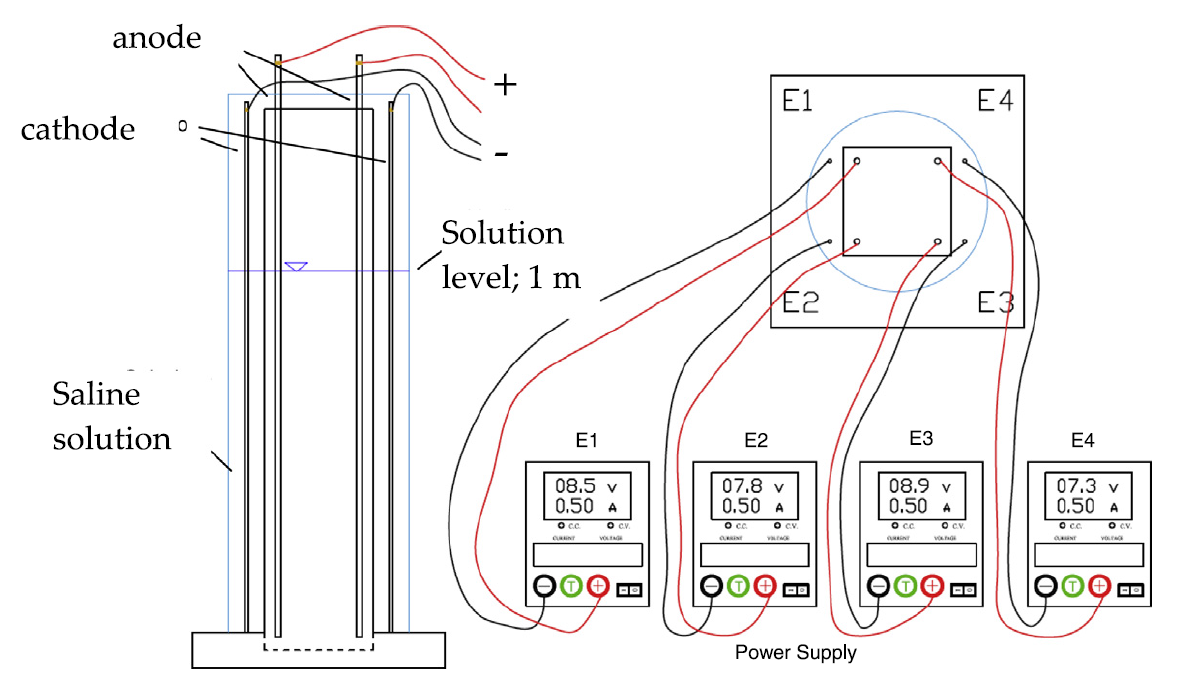
\includegraphics[width=0.7\textwidth]{Chapter-3/figs/Meda_Corrosion}
	\caption{Force displacement response of RC corroded columns \cite{Meda2014}}
	\label{fig:Meda_RC_CorrosionProc}
\end{figure}

The resulting force displacement response of these experiments is shown in \fref{fig:Meda_FD}. It can be seen that there is a reduction of he strength of the system and displacement capacity. 

\begin{figure}[htbp]
	\centering
	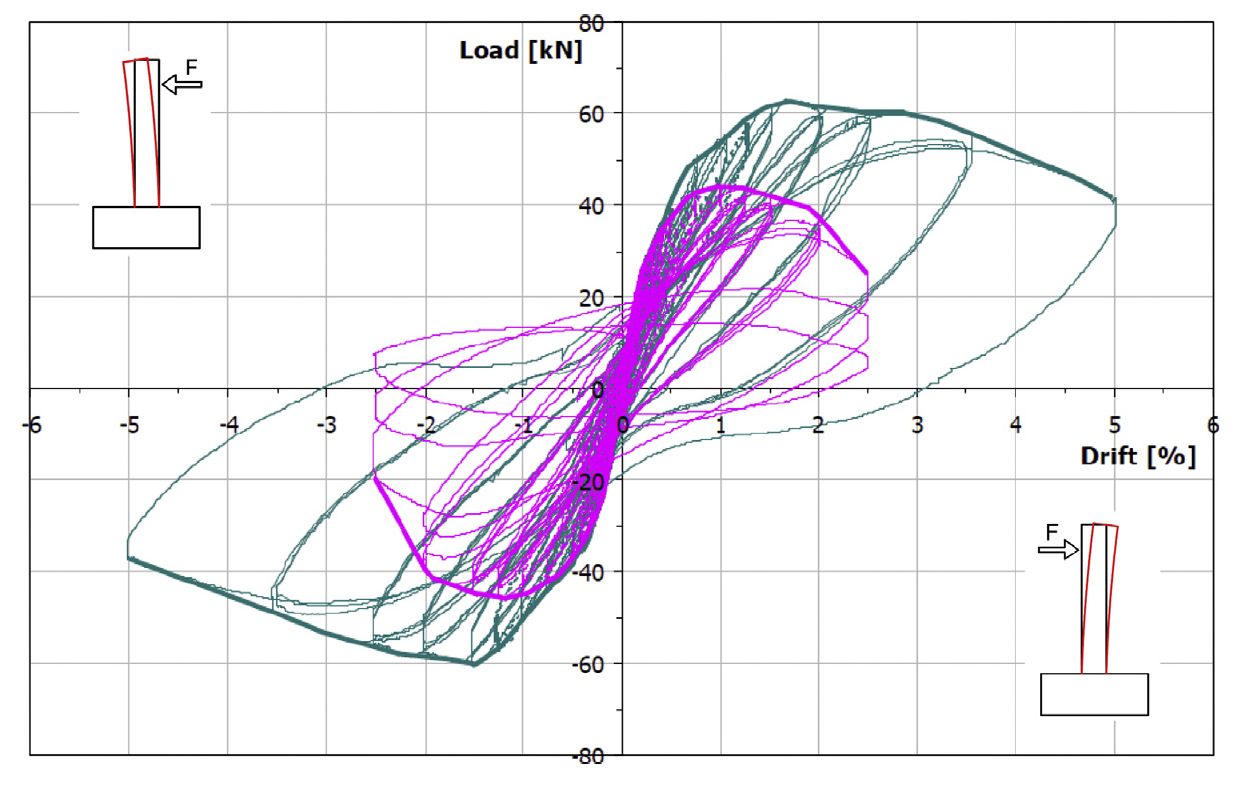
\includegraphics[width=0.7\textwidth]{Chapter-3/figs/Meda_F-D_01}
	\caption{Corrosion process for RC column \cite{Meda2014}}
	\label{fig:Meda_FD}
\end{figure}

As stated in the previous section the mechanical properties of steel are affected by corrosion. In the previous studies \cite{Meda2014} the authors performed tension tests on corroded reinforcing steel. In these tests a reduction in the mechanical properties of steel was observed as well as a reduction in the rupture strain $\varepsilon_{srup}$, see \fref{fig:Meda_RebarTest}. 

\begin{figure}[htbp]
	\centering
	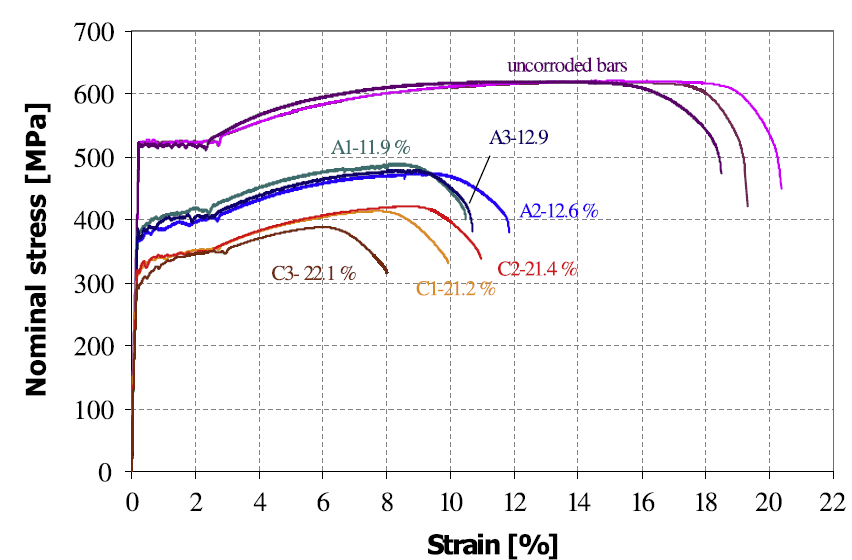
\includegraphics[width=0.7\textwidth]{Chapter-3/figs/Meda_StressStrain}
	\caption{Corroded rebars stress-strain curves \cite{Meda2014}}
	\label{fig:Meda_RebarTest}
\end{figure}

While these studies show how corroded RC columns behave under cyclic loading, they did not consider the generation of the protective film due to the alkaline environment of the concrete. This film can modify the mechanical properties of corroded steel. In addition, the accelerated corrosion process used a 3\% $NaCl$ concentration solution while the chloride attack in concrete usually has a 1.0\% - 1.5\% concentration of the same chloride. Therefore the results obtained from these studies do not accurately represent the actual conditions of corroded RC columns. Thus, an experimental campaign is proposed that will provide results on the mechanical behavior of corroded reinforcing steel inside concrete. This is discussed in the following subsection.

\section{Proposed experimental campaign}

As explained in the previous section the steel inside concrete generates a protective film and after chloride attack reaches the surface of the steel, this protective film starts to be eliminated. This same process will be simulated through the experimental campaign outlined here:

\begin{enumerate}
	\item Passivation of the reinforcing steel
	\item Accelerated corrosion  of Reinforcing Steel
	\item Tension tests
	\item Buckled bar tension (BBT) test
\end{enumerate}

\textbf{Passivation of reinforcing steel}

Methods to generate the passive film on the reinforcing steel surface are available in the literature \cite{Ghods2010}. According to this study, it is possible to generate the passivation process in the same way as it occurs in reinforcing steel embedded in concrete by using an alkaline porous solution. The authors, studied ten different porous solutions, out of which five had all the alkali oxides that exist in the cement. Of these five solutions, the one that showed better performance in the quality of the protective oxides grown on rebar is shown here with its corresponding concentrations:

\begin{itemize}
	\item Saturated calcium hydroxide $Ca(OH)_2$
	\item Sodium hydroxide $Na(OH)$ (4.00 g/l)
	\item Potassium hydroxide $(OH)$ (11.22 g/l)
	\item Calcium sulfate dihydrate $Ca(SO)_4 + 2H_2O$ (13.77 g/l)
\end{itemize}

This is the solution that will be used in this research to generate the passive film on the specimens.

To generate the passivation of the reinforcing steel, the rebars will be placed in the pore solution for a minimum of 8 days. Anodic polarization tests will be measured on the rebars to determine the passive current density. A figure of this process is shown in \fref{fig:RebarPassivation}. In addition, the ends of the rebars will be protected to prevent corrosion in these zones of the specimens, the protection at the ends is based on the standard ASTM G109-07 with some alterations. Figures \fref{fig:RebarSpecimenGeomtry} and \fref{fig:RebarEndsProtection} show the specimen geometry and the preparation of the ends of the rebars.

\begin{figure}[htbp]
	\centering
	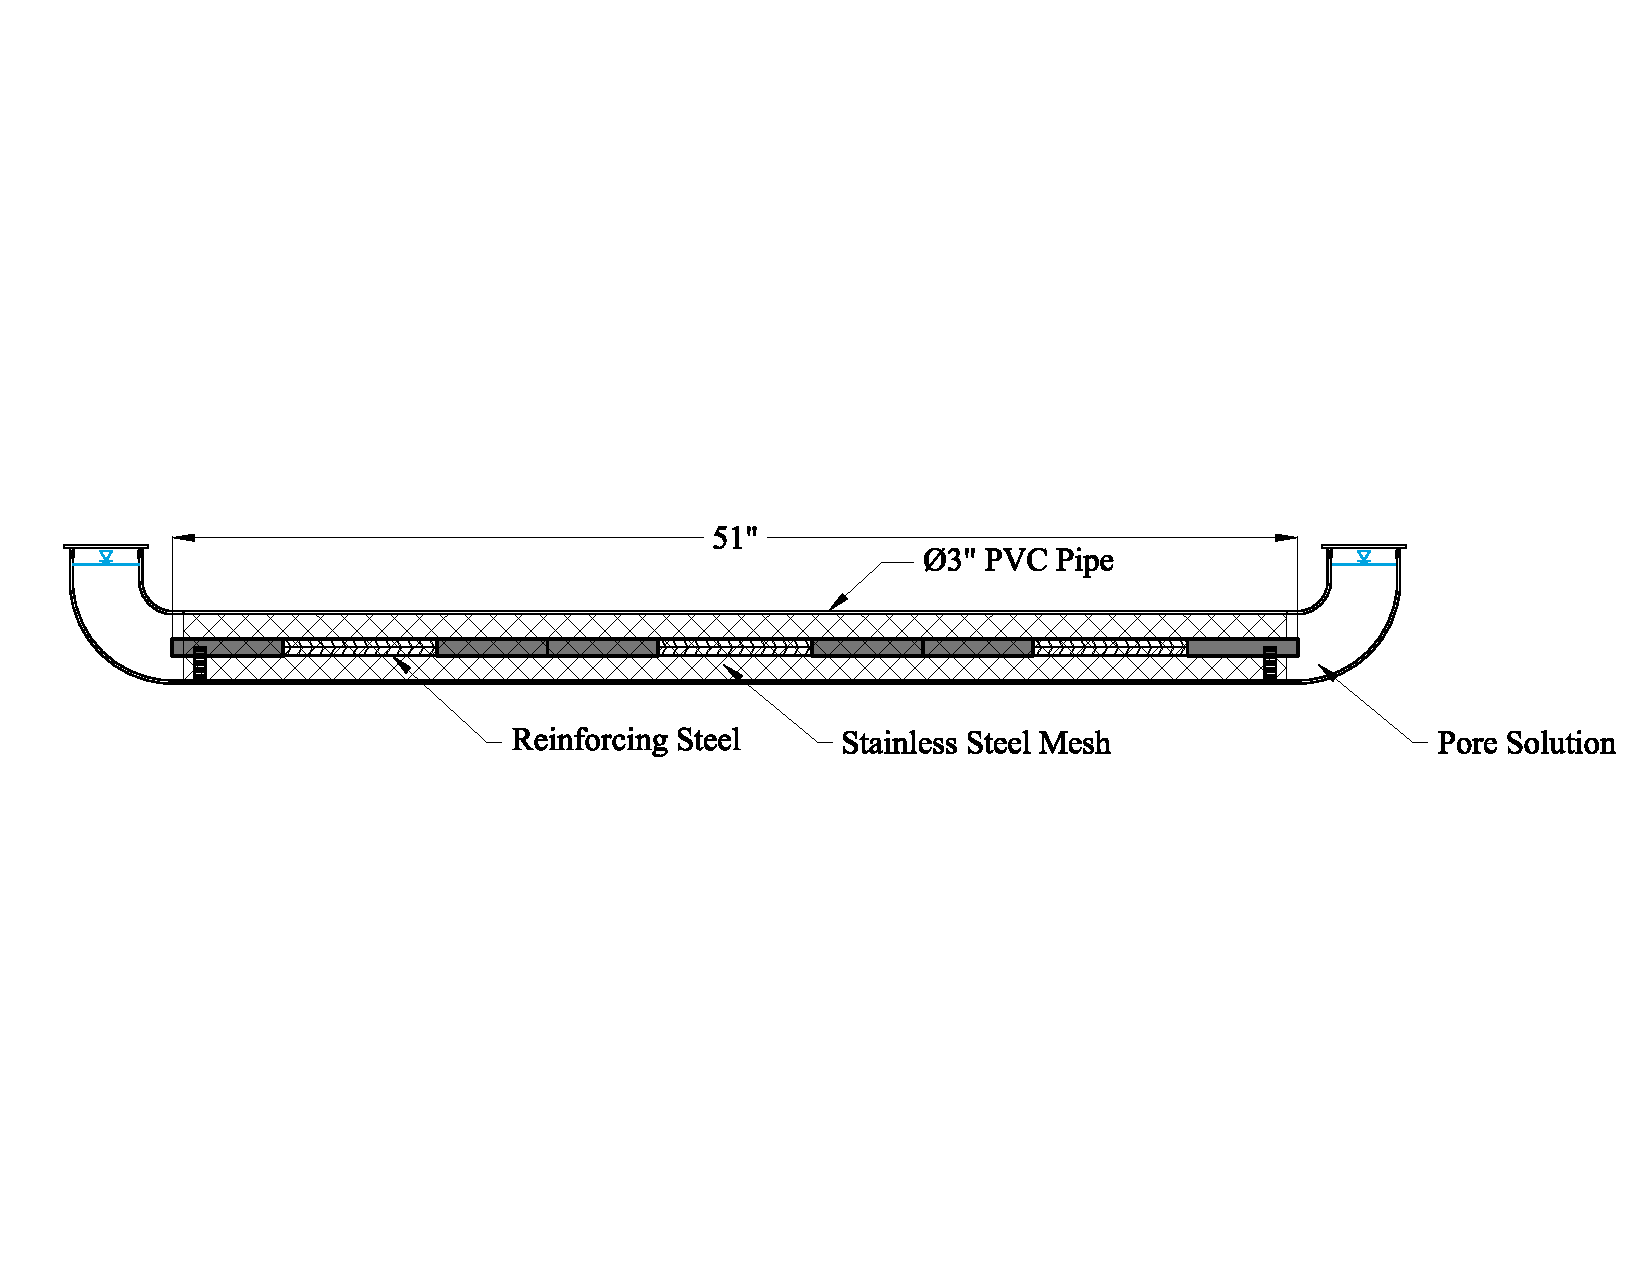
\includegraphics[width=1.0\textwidth]{Chapter-3/figs/AnodicPolarization_01}
	\caption{Rebars Passivation Process in Calcium Hydroxyde Pore Solution}
	\label{fig:RebarPassivation}
\end{figure}

\begin{figure}[htbp]
	\centering
	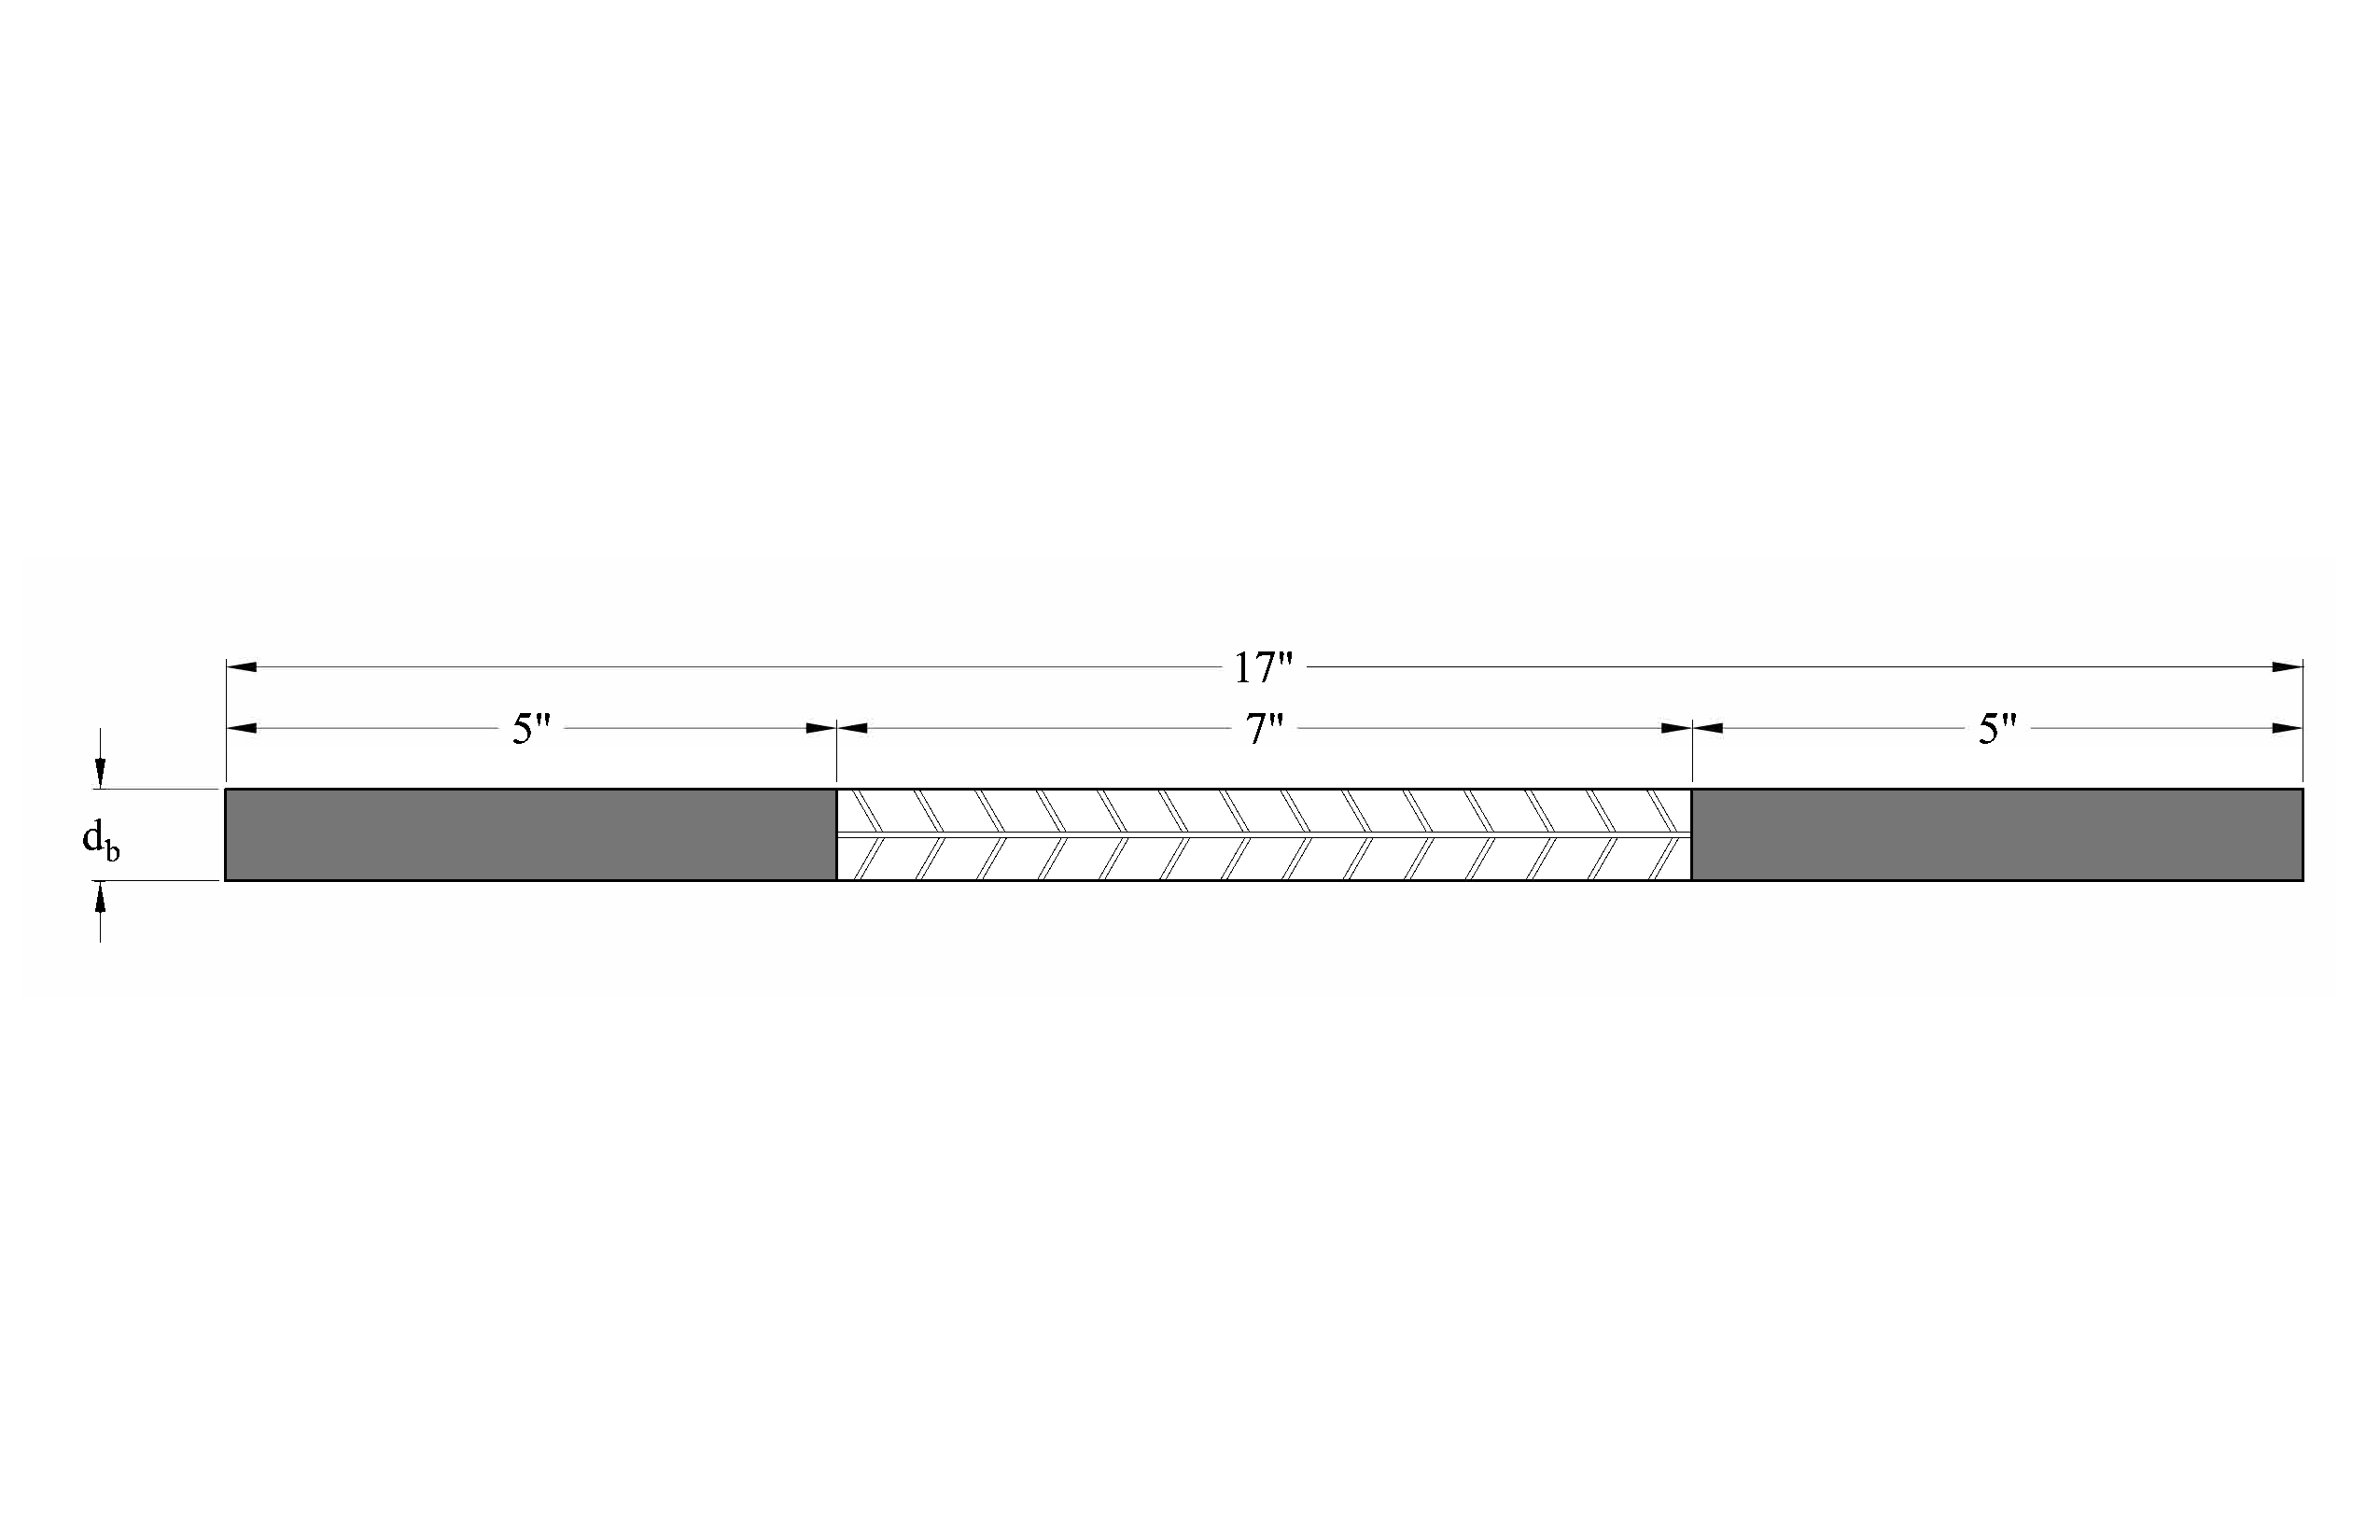
\includegraphics[width=0.9\textwidth]{Chapter-3/figs/RebarSamples}
	\caption{Rebar Specimen Geometry}
	\label{fig:RebarSpecimenGeomtry}
\end{figure}

\begin{figure}[htbp]
	\centering
	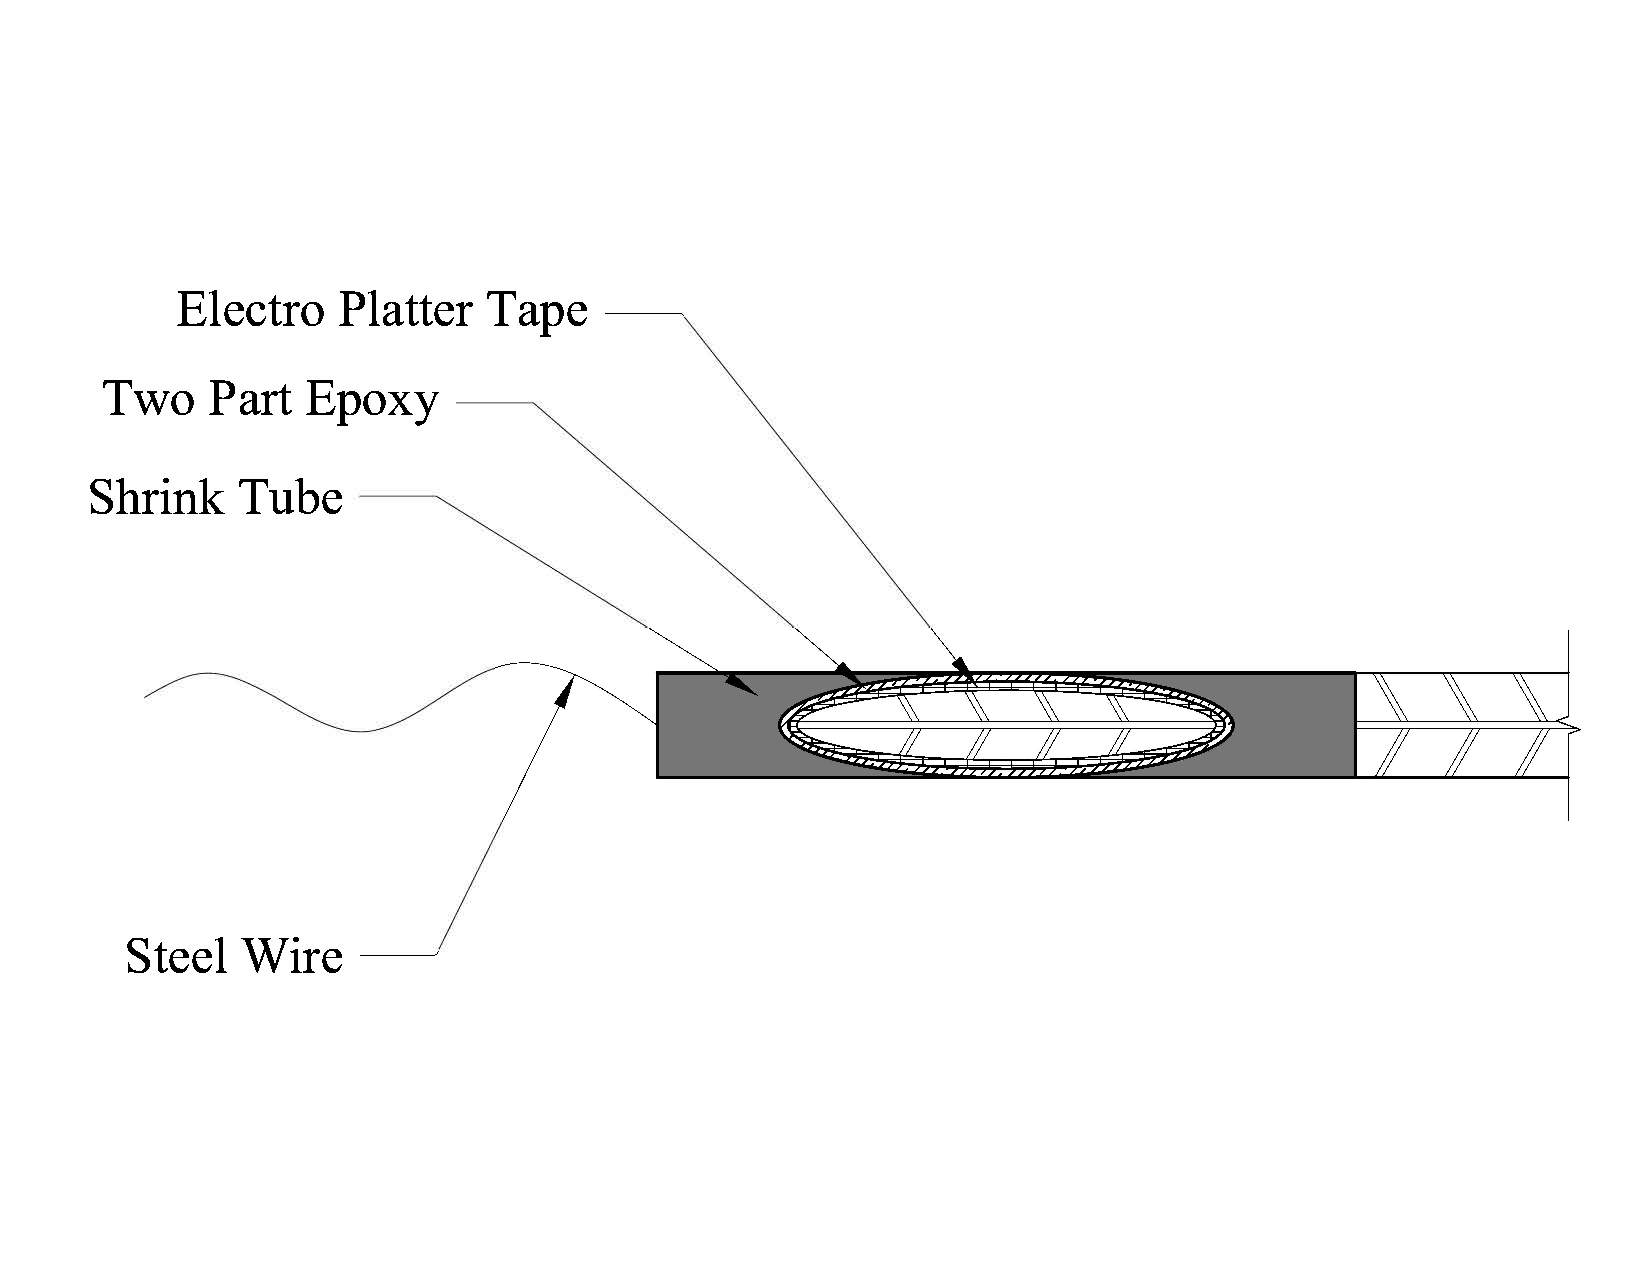
\includegraphics[width=0.9\textwidth]{Chapter-3/figs/Rebar_Ends}
	\caption{Rebars Ends Protection}
	\label{fig:RebarEndsProtection}
\end{figure}


\textbf{Accelerated corrosion  of Reinforcing Steel}

The accelerated corrosion will be done by using a galvanic cell. Different studies \cite{Ghods2010} have shown that for rebars with pasive films a concentration of 0.3 Moles of sodium chloride ($NaCl$) will start the depassivation process on the rebars. In the study presented here, the specimens will be subjected to a current of 5mA equivalent to $47\mu A/cm^2$. This current is sustained for a period of time according to Faraday's Law until the desired level of corrosion is reached.

\begin{equation}
	t=\frac{\lambda m_{loss} \eta_{specimen} C_{faraday}}{i M_{specimen}}
	\label{eq.FaradayEq}
\end{equation}

\begin{figure}[htbp]
	\centering
	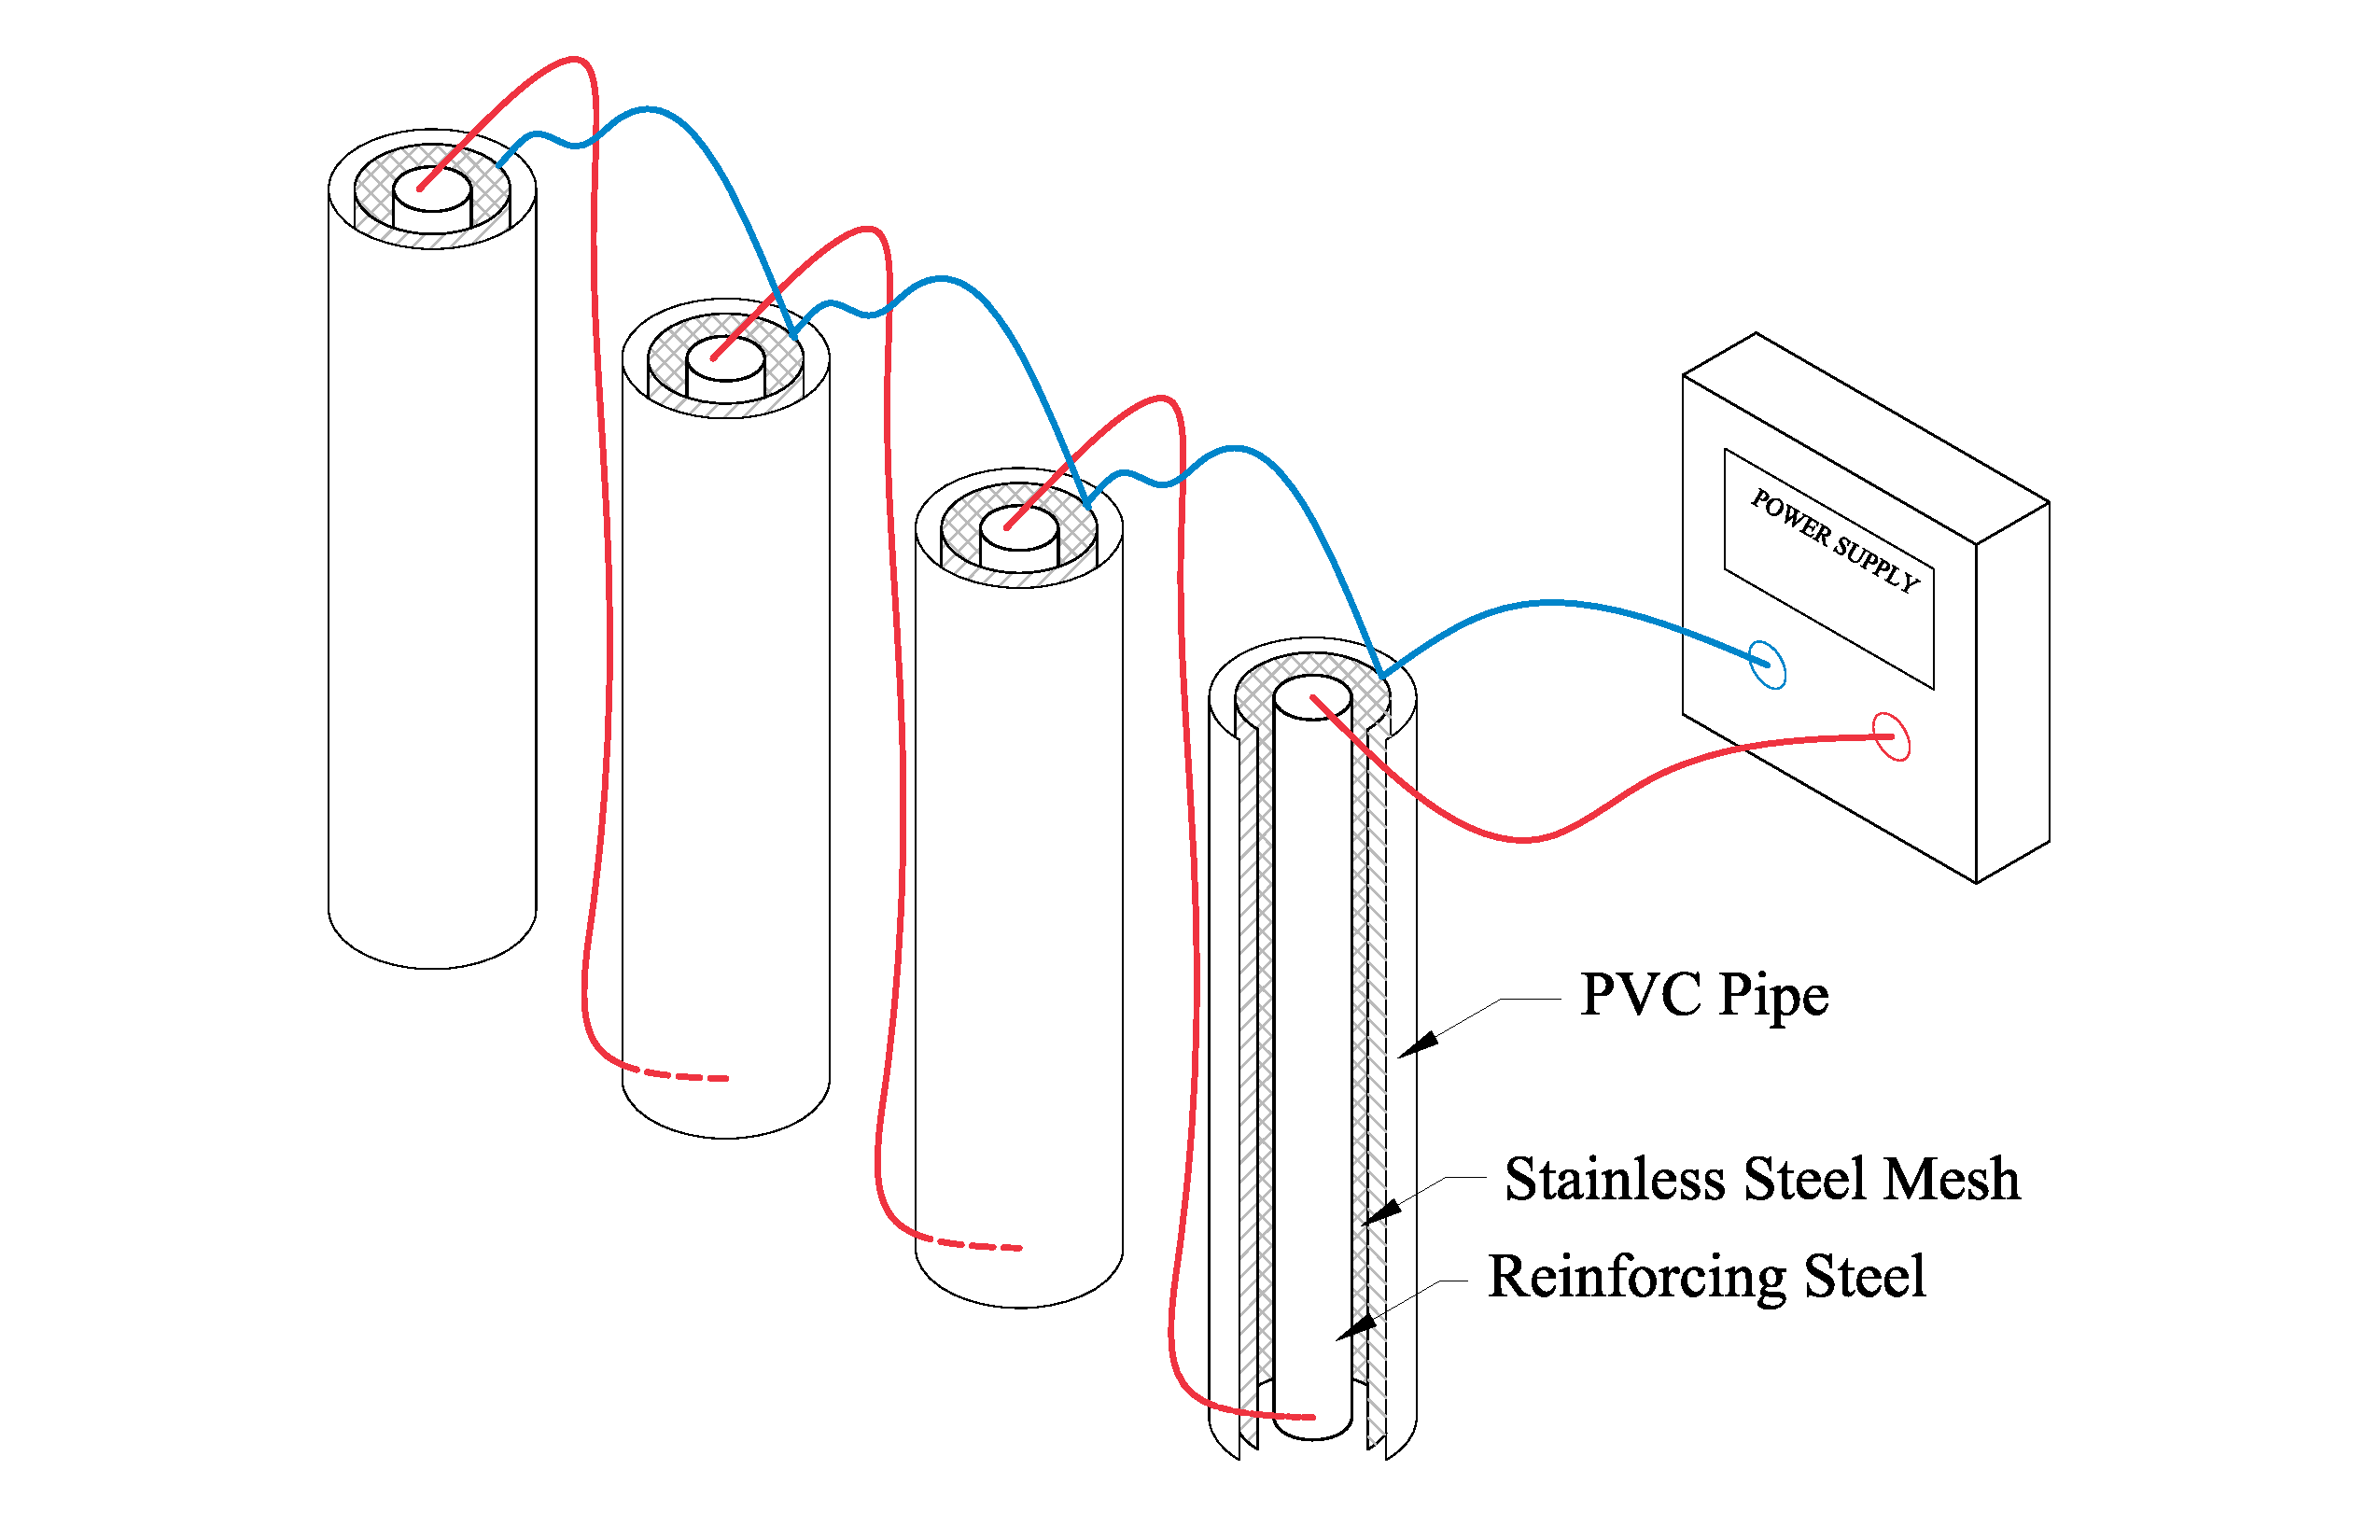
\includegraphics[width=0.9\textwidth]{Chapter-3/figs/AcceleratedCorrosionProcedure}
	\caption{Accelerated corrosion process}
	\label{fig:AcceleratedCorrosion}
\end{figure}

For the different corrosion levels the current and the time of application is shown in Table \ref{tab:AcceleratedCorrosionTime}. 

\begin{table}[htbp]
	\caption{Accelerated corrosion times in 3/4" rebar}
	\label{tab:AcceleratedCorrosionTime}
	\centering	
		\begin{tabular}{|l|c|c|}
		\hline
		Corrosion Level (CL) & Mass loss (g)   & time(days)     \\  \hline	
		5\%                  & 1.12            & 9  \\  \hline	
		10\%                 & 2.24            & 18 \\  \hline	
		15\%                 & 3.36            & 27 \\  \hline	
		20\%                 & 4.47            & 36 \\  \hline	
		25\%                 & 5.59            & 45 \\  \hline	
		\end{tabular}
\end{table}


\textbf{Tension Tests}

A series of tension tests will be performed according to ASTM A706. The main objective of this tests is to evaluate differences in the stress-strain behavior of corroded reinforcing steel. This will determine if there is any reduction in the ductility of steel for this condition.
\newline

\textbf{Buckled Bar Tension (BBT) Test}

One of the limit states that control performance-based design is buckling of reinforcing steel, recent tests have been developed to determine the critical bending strain of buckling of reinforced steel \cite{Barcley2019}. The buckled bar tension (BBT) test simulates bending and tension strain demands on a buckled bar, to determine critical bending strain in buckled rebars. However, the results shown in their study were developed for rebars in pristine condition, therefore, it is necessary to check if the available expressions are valid for corroded reinforcing steel.

The buckled bar tension test consists in:

\begin{enumerate}
	\item Compress a rebar specimen up to a certain level of compression strain such that the rebar will show buckling
	\item The rebar is then pulled until rupture
	\item Repeat the process for different levels of compression strains 
\end{enumerate}

This test is proposed for different levels of corrosion such that any changes on the behavior are studied and incorporated in the analytical model. The test procedure is shown in \fref{fig:BBTseq}. In addition the proposed test matrix is shown in Table \ref{tab:Test Matrix}.

\begin{figure}[htbp]
	\centering
	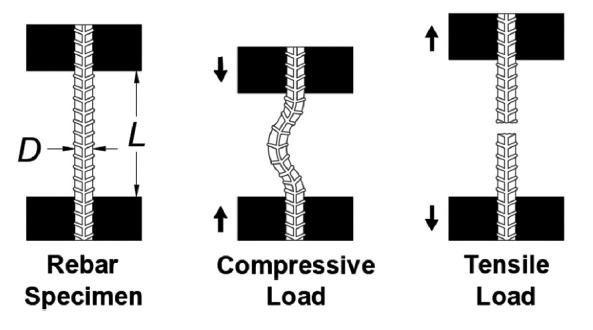
\includegraphics[width=0.7\textwidth]{Chapter-3/figs/BBT_Sequence}
	\caption{BBT Test sequence\cite{Barcley2019}}
	\label{fig:BBTseq}
\end{figure}

% Please add the following required packages to your document preamble:
% \usepackage{multirow}
% \usepackage[table,xcdraw]{xcolor}
% If you use beamer only pass "xcolor=table" option, i.e. \documentclass[xcolor=table]{beamer}
\begin{table}[]
	\caption{Corroded Rebar Test Matrix}
	\label{tab:Test Matrix}
	\centering	
	\begin{tabular}{|c|c|c|c|}
	\hline
	\multicolumn{4}{|c|}{\cellcolor[HTML]{CC0000}{\color[HTML]{FFFFFF} Corroded BBT Test Matrix}}                                               \\ \hline
	\multicolumn{1}{|l|}{Test}     & \multicolumn{1}{l|}{Diameter of Bar} & \multicolumn{1}{l|}{CL (\%)} & \multicolumn{1}{l|}{Number of Tests} \\ \hline
	                               &                                      & 0                            & 3                                    \\ \cline{3-4} 
	                               &                                      & 5                            & 3                                    \\ \cline{3-4} 
	                               &                                      & 10                           & 3                                    \\ \cline{3-4} 
	                               &                                      & 15                           & 3                                    \\ \cline{3-4} 
	                               &                                      & 20                           & 3                                    \\ \cline{3-4} 
	\multirow{-6}{*}{Tension Test} & \multirow{-6}{*}{\#6}                & 25                           & 3                                    \\ \hline
	                               &                                      & 0                            & 6                                    \\ \cline{3-4} 
	                               &                                      & 5                            & 6                                    \\ \cline{3-4} 
	                               &                                      & 10                           & 6                                    \\ \cline{3-4} 
	                               &                                      & 15                           & 6                                    \\ \cline{3-4} 
	                               &                                      & 20                           & 6                                    \\ \cline{3-4} 
	\multirow{-6}{*}{BBT Test}     & \multirow{-6}{*}{\#6}                & 25                           & 6                                    \\ \hline
	\end{tabular}
\end{table}
